
\documentclass{standalone}
\usepackage{tikz}

% Définir le nombre d'états
\def\N{3}
% Définir les couleurs basées sur la palette Cubhelix
\definecolor{cubhelix0}{RGB}{218, 59, 70}
\definecolor{cubhelix1}{RGB}{58, 133, 75}
\definecolor{cubhelix2}{RGB}{63, 127, 147}

% Définir un style personnalisé pour les étiquettes des flèches
\tikzset{
    arrow label/.style={
        font=\Large\sffamily,
        inner sep=3pt
    }
}

\begin{document}

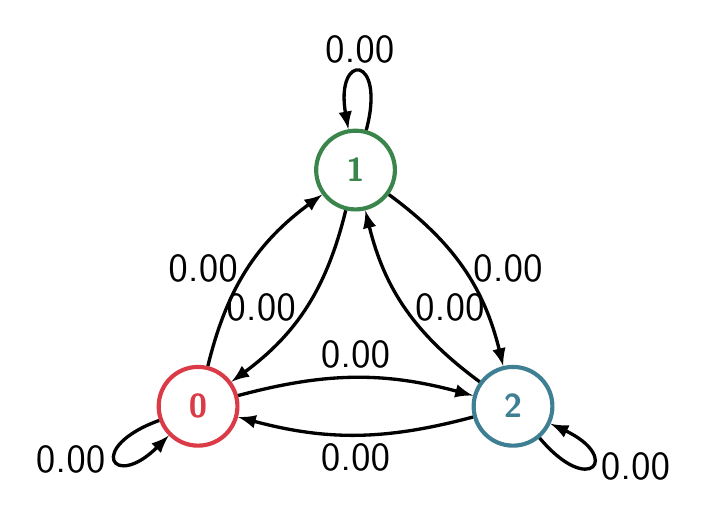
\begin{tikzpicture}[->, auto, thick, node distance=4cm, >=latex] 

    \tikzstyle{state0} = [
        circle, 
        draw=cubhelix0, 
        line width=1.5pt, 
        text=cubhelix0, 
        minimum size=1cm, 
        font=\large\sffamily\bfseries
    ]
    \tikzstyle{state1} = [
        circle, 
        draw=cubhelix1, 
        line width=1.5pt, 
        text=cubhelix1, 
        minimum size=1cm, 
        font=\large\sffamily\bfseries
    ]
    \tikzstyle{state2} = [
        circle, 
        draw=cubhelix2, 
        line width=1.5pt, 
        text=cubhelix2, 
        minimum size=1cm, 
        font=\large\sffamily\bfseries
    ]

    % Créer les nœuds
    \node[state0] (0) at (0,0) {0};
    \node[state1] (1) at (2,3) {1};
    \node[state2] (2) at (4,0) {2};

    % Dessiner les arêtes avec des flèches améliorées
    \path[->, very thick, >=latex, draw=black] 
        (0) edge [loop left, distance=1cm, out=200, in=225] node[arrow label, left] {0.00} (0)
            edge [bend left=20] node[arrow label, left] {0.00} (1)
            edge [bend left=15] node[arrow label, above] {0.00} (2)
        (1) edge [loop above, distance=1cm, out=75, in=100] node[arrow label, above] {0.00} (1)
            edge [bend left=20] node[arrow label, left] {0.00} (0)
            edge [bend left=20] node[arrow label, right] {0.00} (2)
        (2) edge [loop right, distance=1cm, out=-50, in=-25] node[arrow label, right] {0.00} (2)
            edge [bend left=15] node[arrow label, below] {0.00} (0)
            edge [bend left=20] node[arrow label, right] {0.00} (1);

\end{tikzpicture}

\end{document}
